% lualatex
\documentclass[10pt]{article}

\usepackage{fontspec}
\usepackage{hyperref}
\usepackage{parskip}
\usepackage{graphicx}
\usepackage{titling}
\usepackage{emoji}
\usepackage[margin=2cm]{geometry}
\usepackage[spanish]{babel}
\usepackage{titlesec}

\newcommand{\github}{
\includegraphics[height=1em]{images/github.png}}
\newcommand{\linkedin}{
\includegraphics[height=1em]{images/linkedin.png}}
\newcommand{\ucsm}{
\includegraphics[height=1em]{images/ucsm.png}}
\newcommand{\afa}{
\includegraphics[height=1em]{images/afa.png}}
\newcommand{\mlk}{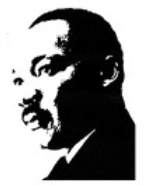
\includegraphics[height=1em]{images/mlk.png}}
\newcommand{\ph}{
\includegraphics[height=1em]{images/ph.png}}
\newcommand{\sbs}{
\includegraphics[height=1em]{images/sbs.png}}
\newcommand{\mov}{
\includegraphics[height=1em]{images/mov.png}}
\newcommand{\alt}{
\includegraphics[height=1em]{images/alt.png}}
\newcommand{\yl}{
\includegraphics[height=1em]{images/yl.png}}
\newcommand{\tec}{
\includegraphics[height=1em]{images/tec.png}}
\newcommand{\unsaac}{
\includegraphics[height=1em]{images/unsaac.png}}
\newcommand{\ucsp}{
\includegraphics[height=1em]{images/ucsp.png}}
\newcommand{\python}{
\includegraphics[height=1em]{images/python.png}}
\newcommand{\octave}{
\includegraphics[height=1em]{images/octave.png}}
\newcommand{\gnu}{
\includegraphics[height=1em]{images/gnu.png}}
\newcommand{\golang}{
\includegraphics[height=1em]{images/golang.png}}
\newcommand{\arch}{
\includegraphics[height=1em]{images/arch.png}}
\newcommand{\debian}{
\includegraphics[height=1em]{images/debian.png}}
\newcommand{\kicad}{
\includegraphics[height=1em]{images/kicad.png}}
\newcommand{\vim}{
\includegraphics[height=1em]{images/vim.png}}
\newcommand{\git}{
\includegraphics[height=1em]{images/git.png}}
\newcommand{\gohugo}{
\includegraphics[height=1em]{images/gohugo.png}}
\newcommand{\gimp}{
\includegraphics[height=1em]{images/gimp.png}}
\newcommand{\inkscape}{
\includegraphics[height=1em]{images/inkscape.png}}
\newcommand{\shotcut}{
\includegraphics[height=1em]{images/shotcut.png}}
\newcommand{\overleaf}{
\includegraphics[height=1em]{images/overleaf.png}}
\newcommand{\linux}{
\includegraphics[height=1em]{images/linux.png}}
\newcommand{\ethree}{
\includegraphics[height=1em]{images/e3.png}}

\setmainfont{Noto Sans}
\setemojifont{Noto Color Emoji}

\hypersetup{
    colorlinks=true,
    linkcolor=green,
    filecolor=magenta,      
    urlcolor=blue,
    pdftitle={Luis Figueroa | CV},
}

\titleformat{\section}
{\Large\bfseries}
{}
{0em}
{}[\titlerule]

\renewcommand{\maketitle}{
    \begin{center}
	{
	    \huge
	    \bfseries
	    \theauthor
	    \\\vspace{.1em}
	}
	\footnotesize
	\emoji{envelope}\href{mailto:luis_figueroa_morales@yahoo.com}{luis\_figueroa\_morales@yahoo.com} --- \emoji{link}\href{https://luisfigueroa.xyz/}{https://luisfigueroa.xyz/} --- \emoji{mobile-phone}971467843 --- \github \href{https://github.com/luisfigueroaa}{/luisfigueroaa} --- \linkedin \href{https://www.linkedin.com/in/luisfigueroaa/}{/luisfigueroaa}
    \end{center}
}

\newcommand{\cvitem}[4] {
    \begin{tabular}{@{}p{.3\textwidth}|p{.68\textwidth}}
	\raggedleft\textbf{{#2}}\\{\footnotesize\textit{#1}} & \ifx&#3&{#4}\else{\bfseries\footnotesize\MakeUppercase{{#3}}}\newline{#4}\fi\\
    \end{tabular}
    }

\title{Curriculum Vitae}
\author{Luis Orlando Figueroa Morales}

\begin{document}
\maketitle

\section{Descripción personal}

Me considero una persona responsable con ganas de aprender cada día algo nuevo, mejorar mis habilidades y perseverar para conseguir mis metas con liderazgo y responsabilidad en cualquier tarea que realice.

Soy capaz de adquirir conocimientos de manera autodidáctica y me gusta compartir lo que sé con las personas que trabajo y convivo.

Cuento con licencia A-1, disponiblidad inmediata ya sea fuera o dentro de la ciudad.

\section{Formación académica}

\cvitem{2014-Act.}
    {\ucsm Universidad Católica de Santa María}
    {}
    {Ingeniería Electrónica}

\cvitem{2020}
    {\afa Alianza Francesa de Arequipa}
    {}
    {Francés}

\cvitem{2006-2010}
    {\mlk Martin Luther King, Jr. School of English}
    {}
    {Inglés}

\section{Experiencia laboral}

\cvitem{2015-2016}
    {\mlk Martin Luther King, Jr. School of English}
    {Instructor de Inglés}
    {Enseñé a niños y jóvenes adultos inglés en nivel básico.}

\cvitem{2017-2019}
    {\ph Pizza Hut}
    {Colaborador en producción de alimentos}
    {Trabajé en el área de producción y atención al cliente.}

\cvitem{2018-2019}
    {\sbs Librería Internacional SBS}
    {Atención al cliente y ventas}
    {Atención al cliente y apoyo en el área de logistica durante el festival literario Hay Festival. También durante campaña escolar en la venta de textos escolares.}

\cvitem{2019}
    {\mov Movistar}
    {Atención al cliente}
    {Atención al cliente y configurador de teléfonos de alta gama. Orientación a los clientes en procesos de reclamos y ventas.}

\cvitem{2021}
    {\alt Altelos Technologies}
    {Engineering Project Assistant}
    {Trabajé en el área de telecomunicaciones como practicante y por contrato, adquiriendo conocimiento en el manejo de servidores y en proyectos de electrónica.}

\section{Voluntariado}

\cvitem{2012-2013}
    {GRASP - God Reaching All Southern Peru}
    {Intérprete}
    {Intérprete del idioma inglés para grupo misionero de Estados Unidos.}

\cvitem{2014}
    {\ethree e3 Partners}
    {Intérprete}
    {Intérprete del idioma inglés para grupo misionero de Estados Unidos.}

\cvitem{2014-2017}
    {\yl Young Life}
    {Voluntario}
    {Apoyo en actividades y campamentos del ministerio de jóvenes Young Life.}

\section{Cursos y capacitaciones}

\cvitem{2021}
    {M.P.B. Control Solutions S.A.C}
    {}
    {Curso de espacilización de Fibra Óptica.}

\cvitem{2022}
    {\tec TECSUP}
    {}
    {Gestión de Servidores con Linux.}

\section{Conferencias y congresos}

\cvitem{2014}
    {\ucsm Universidad Católica de Santa María}
    {}
    {Congreso Internacional de Ingeniería Electrónica.}

\cvitem{2015}
    {\ucsm Universidad Católica de Santa María}
    {}
    {Congreso Internacional de Ingeniería Telecomunicaciones.}

\cvitem{2016}
    {\ucsm Universidad Católica de Santa María}
    {}
    {Congreso Internacional de Ingeniería Electrónica.}

\cvitem{2017}
    {\unsaac Universidad Nacional San Antonio de Abad del Cusco}
    {}
    {INTERCON (International Congress on Electronics, Electrical Engineering and Computing) - Cusco.}

\cvitem{2018}
    {\ucsm Universidad Católica de Santa María}
    {}
    {Congreso Internacional de Ingeniería Electrónica.}

\cvitem{2019}
    {\ucsm Universidad Católica de Santa María}
    {}
    {Congreso Internacional de Ingeniería Electrónica.}

\cvitem{2019}
    {\ucsp Universidad Católica San Pablo}
    {}
    {Workshop de Microondas, Antenas y Sensores IEEE.}

\section{Idiomas}

\begin{itemize}
    \begin{minipage}{0.5\linewidth}
    \item \emoji{flag-united-states}\textbf{Inglés}: Intermedio alto
    \end{minipage}
    \begin{minipage}{0.5\linewidth}
    \item \emoji{flag-france}\textbf{Francés}: Básico a intermedio
    \end{minipage}
\end{itemize}

\section{Lenguajes de programación}

\begin{itemize}
    \begin{minipage}{0.5\linewidth}
	\item C
	\item C++
	\item \python Python
	\item Assembly
    \end{minipage}
    \begin{minipage}{0.5\linewidth}
	\item \octave Matlab/GNU Octave
	\item \gnu Bash/shell
	\item \golang Go
	\item Markup Languages: \LaTeX, Markdown, HTML, CSS.
    \end{minipage}
\end{itemize}

\section{Software que uso}

\begin{itemize}
    \item \textbf{Sistema Operativo}: \gnu\linux GNU/Linux.
    \item \textbf{Distribuciones}: \arch\textbf{Arch Linux} (en mi computadora personal) y \debian\textbf{Debian} (en mi servidor).
    \item \textbf{Automatización de Diseño electrónico}: \kicad Kicad y Ngspice.
    \item \textbf{Editor de textos}: \vim Vim (Neovim).
    \item \textbf{Otro software que también utilizo}: Tengo experiencia usando \git \textbf{Git} para el control de versiones de proyectos y archivos personales. Uso el framework de \gohugo \textbf{Hugo} para creación de sitios web. Tengo práctica en software de edición gráfica como \gimp \textbf{GIMP}, \inkscape \textbf{Inkscape} e \textbf{Imagemagick},y para la edición de video utilizo los software \textbf{FFMPEG} y \shotcut \textbf{Shotcut}.
\end{itemize}

\section{Contáctame}

Para contactarme para trabajo (por contrato u honorarios) y/o proyecto puedes enviarme un correo electrónico a \emoji{envelope}\href{mailto:luis_figueroa_morales@yahoo.com}{luis\_figueroa\_morales@yahoo.com} o a mi celular \emoji{mobile-phone}971467843.

\section{Acerca de mi CV}

Todo mi CV está desarrollado en mi entorno de Vim con \LaTeX{} y el código fuente se encuentra en \overleaf\href{https://www.overleaf.com/read/tzqrsyfkpskn}{Overleaf}.

\end{document}
